\documentclass{article}
\usepackage{tikz}
\usepackage{graphicx} % Required for inserting images

\title{PAMPI A01}
\author{Sriram katta}
\date{October 2025}

\begin{document}

\maketitle

\section{Amdahl scaling law}
Amdahl law assumes scalable resources, so we only consider the points at process counts of 20,40,60, and 80

\begin{figure}[h]
\centering
\begin{tikzpicture}
    \node[anchor=south west,inner sep=0] (image) at (0,0) {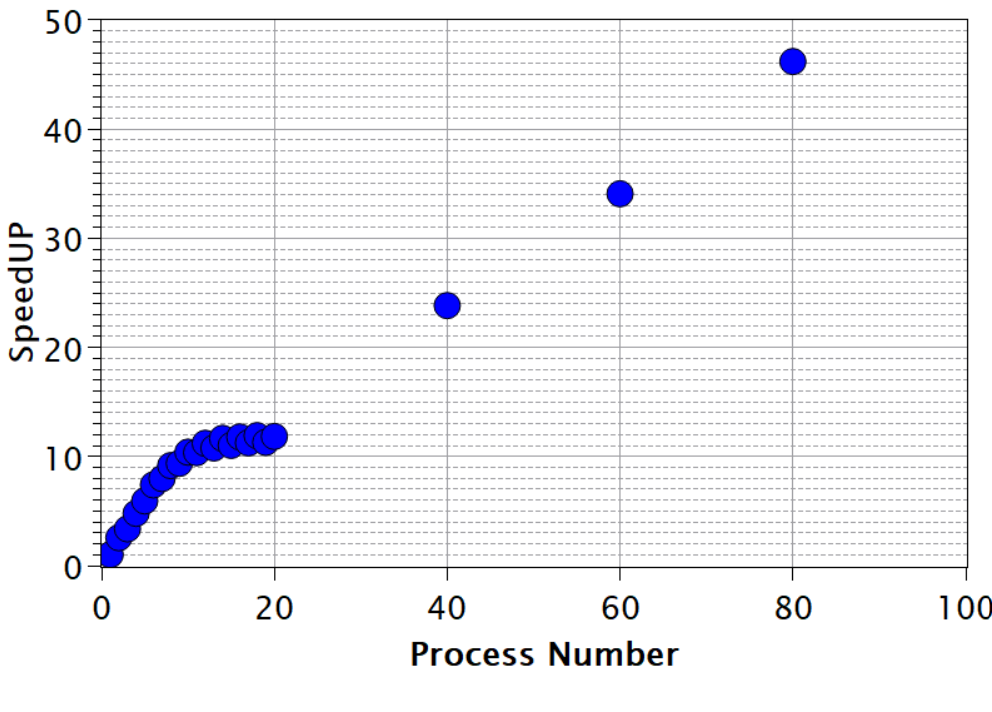
\includegraphics[width=\textwidth]{media/speedup.png}};

    \begin{scope}[x={(image.south east)},y={(image.north west)}]

    \draw[red, thick] (0.28,0.38) circle [radius=0.03];
    \draw[red, thick] (0.455,0.57) circle [radius=0.03];
    \draw[red, thick] (0.625,0.72) circle [radius=0.03];
    \draw[red, thick] (0.80,0.92) circle [radius=0.03];    
    \end{scope}
\end{tikzpicture}
\caption{Image with shapes drawn on top.}
\end{figure}

\begin{table}[h!]
    \centering
    \begin{tabular}{c|c}
         process count & Speedup \\
         20 & 12 \\
         40 & 24 \\
         60 & 34 \\
         80 & 46
    \end{tabular}
    \caption{process count with respective speedup}
    \label{tab:procvsspeedup}
\end{table}

\begin{equation}
    S(N)=\frac{T(1)}{T(N)}=\frac{1}{1+\frac{1-s}{N}}
\end{equation}
we can observe that
\begin{equation}
    S(N) \propto \frac{1}{T(N)}
\end{equation}

resulting in
\begin{equation}
    \frac{S(N)}{S(1)}=\frac{1}{s+\frac{1-s}{N}}
\end{equation}

\[
\frac{46}{12}=\frac{1}{s+\frac{1-s}{4}}
\]

\[ 
s = \frac{1}{69} = 1.44\%
\]

the serial fraction is around $1.44\%$ 

\end{document}
